\chapter{Analyse von artverwandten Spielen zur Konzeptentwicklung}\label{sec:analysis}
\say{Connecting-Minds} besitzt ein grundlegendes Spielkonzept, das durch die Analyse von artverwandten Spielen aus dem Kapitel \emph{\nameref{sec:sota}} und weiteren Spiele, die durch ihr Spieldesign als Vorlage für die Anwendungen von \say{Connecting-Minds} als Vorlage dienen können, erweitert werden soll.

Außerdem soll durch durch die Ergebnisse der Analyse die Forschungsfrage \emph{\say{Welche spezifischen Eigenschaften muss eine solche Umgebung aufweisen und welche Kommunikationsparameter werden dabei angesprochen?}} beantwortet werden können.

\section{Methodik}
Zur systematischen Untersuchung der artverwandten Spiele wurde ein mehrstufiges, eigens entwickeltes Analyseraster verwendet. Dieses gliedert sich in folgende Abschnitte:

\subsection{Visuelle Analyse}
Im visuellen Design wurde zunächst der Fokus auf sichtbare Rätsel- und Hinweiselemente der Spiele gelegt. Dabei wurden diese jeweils im Bild markiert. Die Markierungen dienten der späteren Auswertung, welche Aspekte dabei auffielen oder welche Arten von Rätseldesign genutzt wurden. Zusätzliche wurden so auch einzelnen Interaktionsflüsse erkannt und aufgereiht.

\subsection{Erstellung eines Diagramms zur Rätselstruktur}
Im zweiten Schritt nach der visuellen Analyse wurden für bestimmte Abschnitte oder das ganze Spiel UML-Ablauf Diagramme angelegt, die den Aufbau und die Verschachtlungen der Rätselelemente aufzeigen sollen. Hierbei wurde sich an der Arbeit von \cite{tim_schafer_grim_1996} orientiert.

\subsection{Deskriptive Übertragung}
Im dritten Schritt wurden Erkenntnisse zum Rätseldesign aus Schritt 1 (Visuelle Analyse) und Schritt 2 (Erstellung des Diagramms) zusammengefasst.

\subsection{Schlussfolgerung}
Im letzten Schritt wurden die Beobachtungen aus den vorangegangenen Schritten in Bezug auf die Konzeptentwicklung von \say{Connecting-Minds} gesetzt und Rückschlüsse in das eigene Konzept eingearbeitet.

\section{Ergebnisse der Analysen}
In den einzelnen Kapiteln werden nun die Analysen zu den Spielen \say{We were here}, \say{We were here too}, \say{The past within}, \say{Tiny Room Stories}, \say{Myrmidon} und \say{Keep Talking and Nobody Explodes} vorgestellt.

\subsection{We were here - Spielreihe}
Es wurde sich hier nur auf die ersten zwei Teile (\say{We were here} und \say{We were here too}) der Spielreihe beschränkt, da der Umfang alle Spiele zu spielen und zu analysieren zu wenig Ertrag ergeben würde und daher in der Breite der Spiele analysiert wurde. Die beiden Spiele werden im Folgenden als ganzes betrachtet, also der gesammte Inhalt des Spiels.

\paragraph{Visuelle Analyse}
Abbildungen \ref{fig:wwh-visuals} in Anhang [Anhang verlinken] und \ref{fig:wwht-visuals} in Anhang [Anhang verlinken] geben einen Einblick in die Analyse der Spieler-Rollen der Spiele. Schnell fällt auf, dass die Rätselelemente der Spiele sehr häufig über Symbole oder Bilder gestaltet wurde, bei denen diese beschrieben werden, richtig ausgewählt und platziert werden müssen. Grundlegend sind die Rätsel in der Spielwelt eingebaut, das bedeutet, dass entweder Symbole an den Wänden zu sehen sind, oder Anweisungen in Textform in der Spielwelt integriert sind. Selten ist es so, dass durch auditives Storytelling oder Texte in Büchern Rätsel gelöst werden müssen. In \say{We were here} fällt zudem auf, dass der \say{Explorer} die eingebauten Rätsel lösen muss und der \say{Librarian} sich in einer Hub befindet, über welchen der zu allen Rätseln die richtige Lösung finden muss. In \say{We were here too} ist es ähnlich. Häufig befindet sich der \say{Peasant} in Räumen mit den Rätseln und der \say{Lord} in den Räumen mit den Lösungen. Allerdings wurde hier öfters auch der \say{Lord} durch das Lösen von Rätseln gefordert. Außerdem befindet er sich nicht in einem zentralen Hub.

\paragraph{Analyse des Rätseldesigns}
Abbildung \ref{fig:wwh-uml} und \ref{fig:wwht-uml} zeigen jeweils die Ablaufdiagramme von \say{We were here} und \say{We were here too}. Auffallend ist, dass in \say{We were here} die Rolle des \say{Librarian}s im Kontext des Rätseldesigns linear verläuft und nur selten verschachtelte Rätsel aufzufinden sind. Grundlegend ist es so, dass der \say{Explorer} auf die Rätsel und Hindernisse trifft, und der \say{Librarian} dafür zuständig ist, die richtigen Antworten zu liefern. Es findet eine sehr eindimensionale Verkettung zwischen den Rollen statt.
In \say{We were here too} lassen sich im Vergleich zum Vorgänger-Teil öfters verkettetes Rätseldesign finden, zum Beispiel in Raum 2 des Spiels. Dies ist jedoch auch in Ausnahmen der Fall, es wiederholt sich ein ähnlicher Aufbau wie im Vorgänger.

\begin{figure}[ht]
\centering
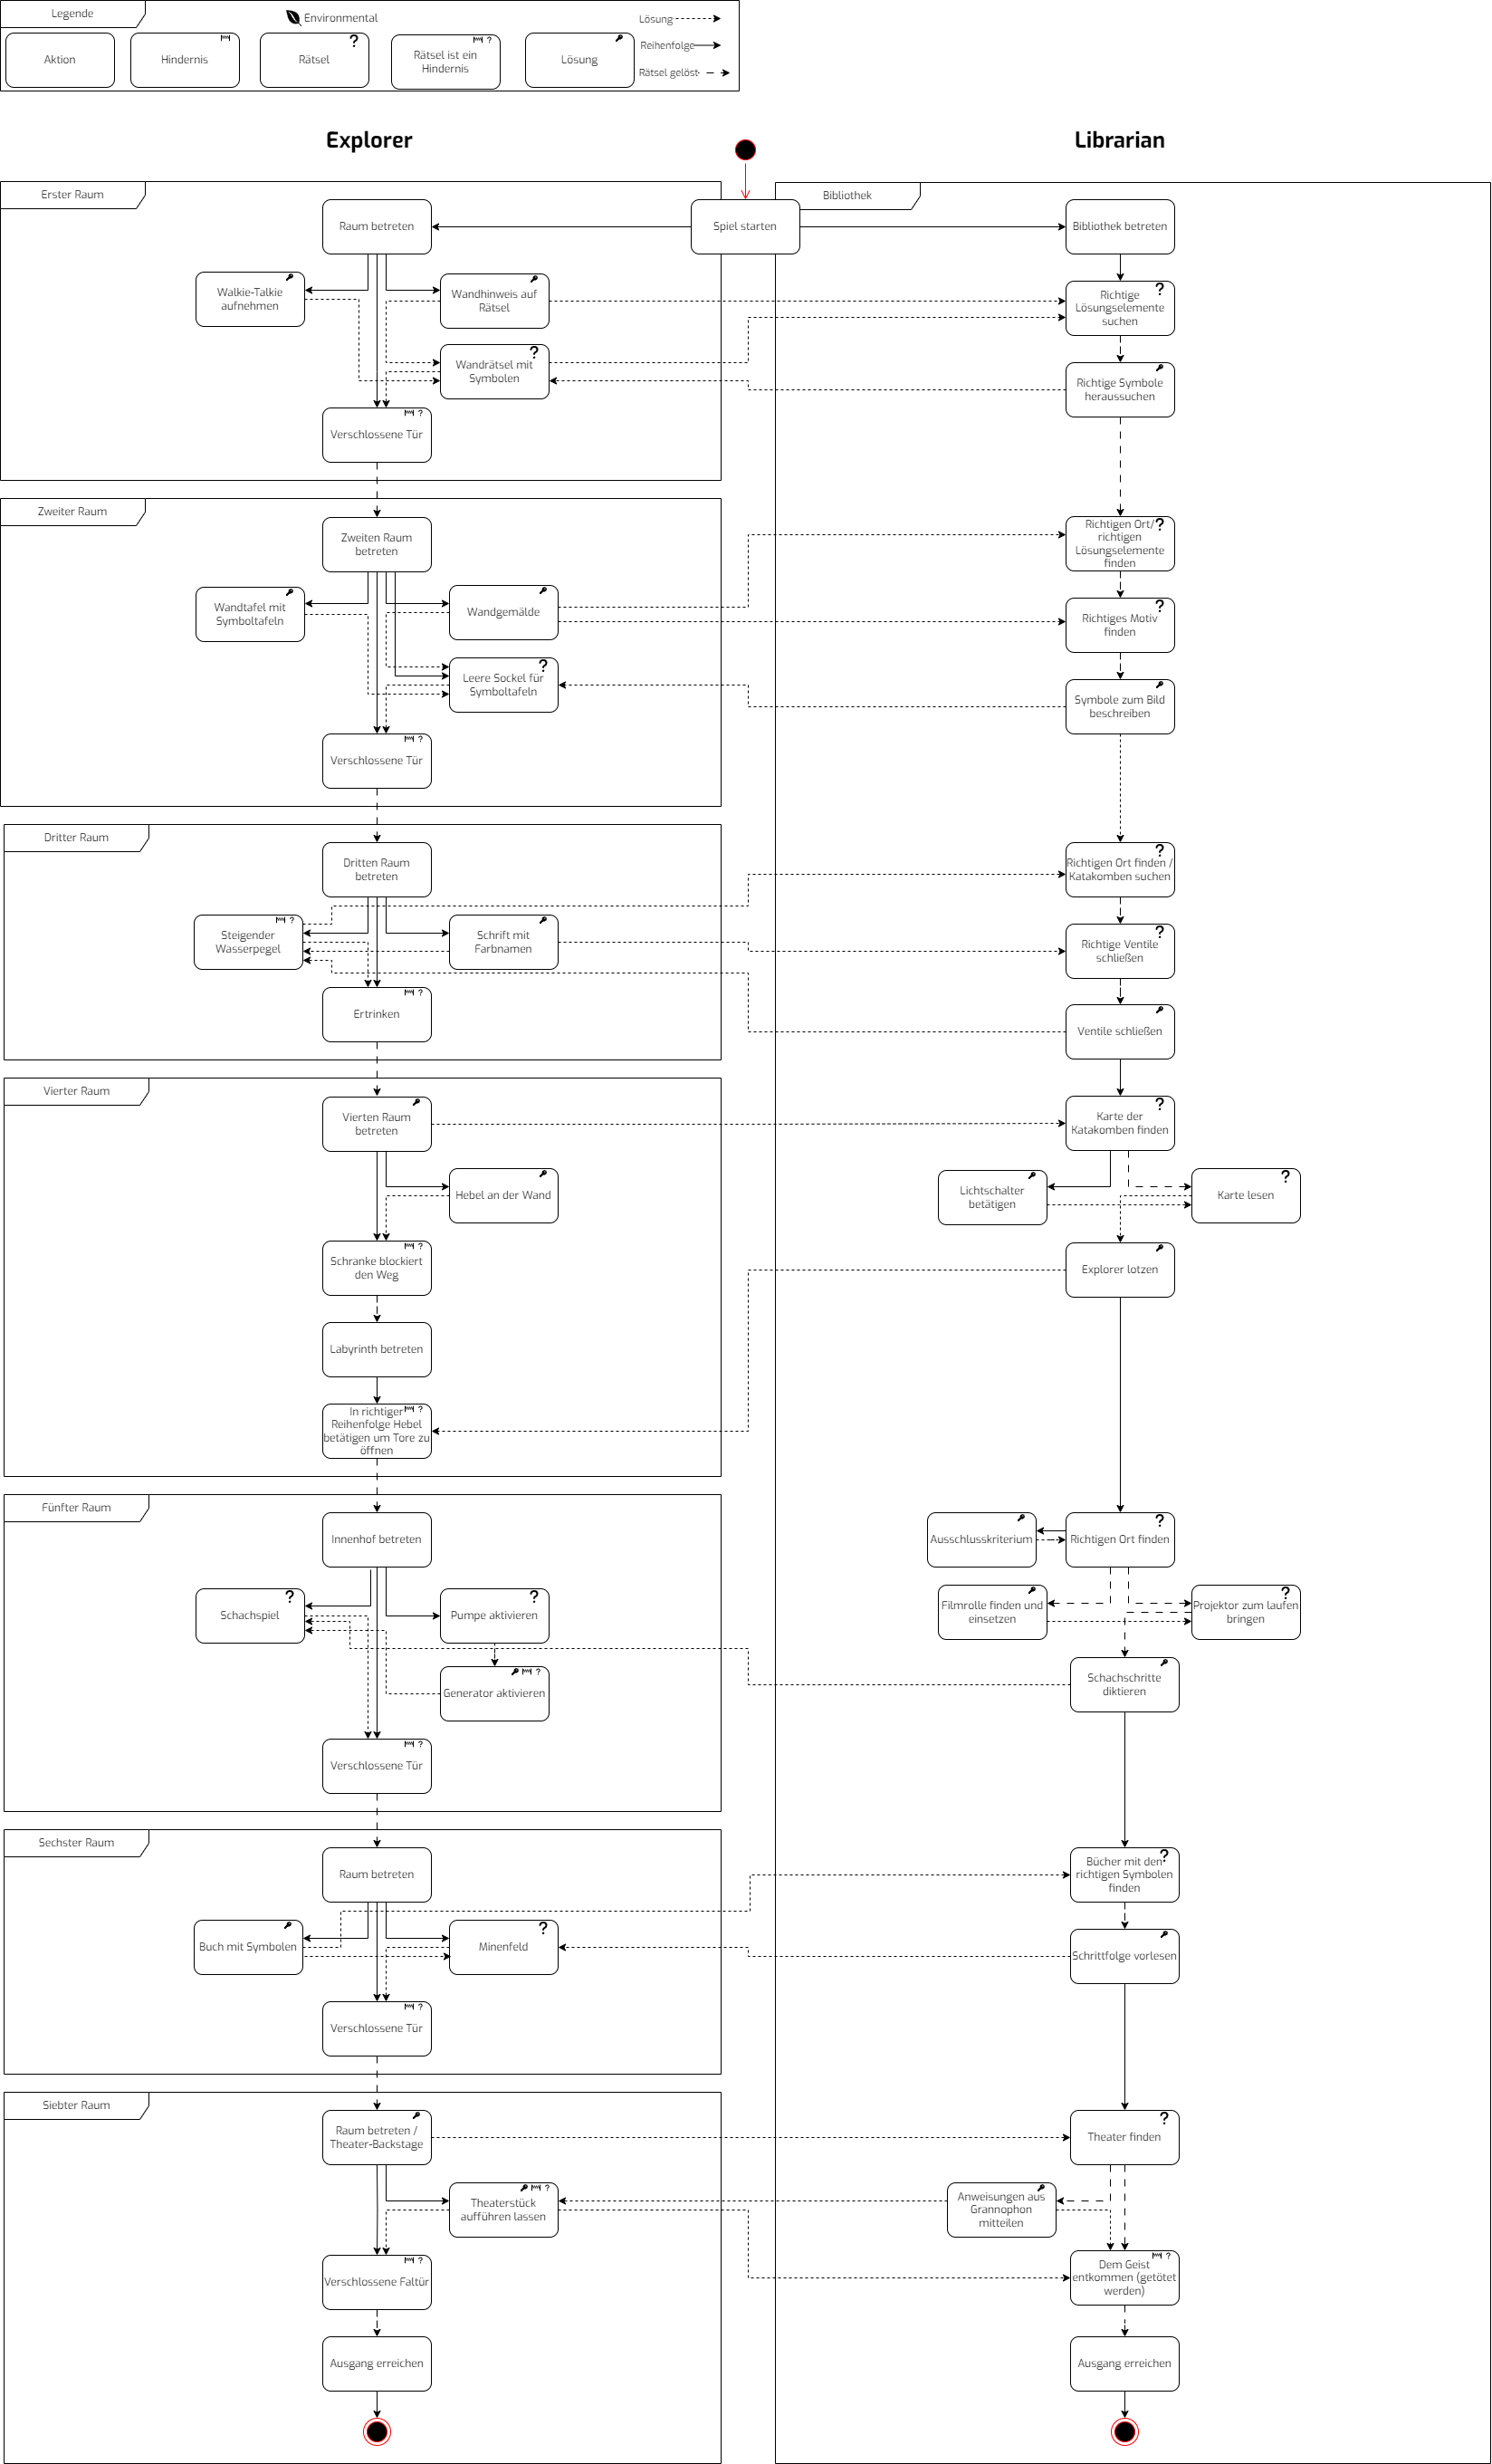
\includegraphics[width=0.8\linewidth]{content/pictures/WeWereHereUML.png}
\caption{Rätseldesign von We were here (Quelle: eigene Darstellung), vollständig in Anhang: }
\label{fig:wwh-uml}
\end{figure}

\begin{figure}[ht]
\centering
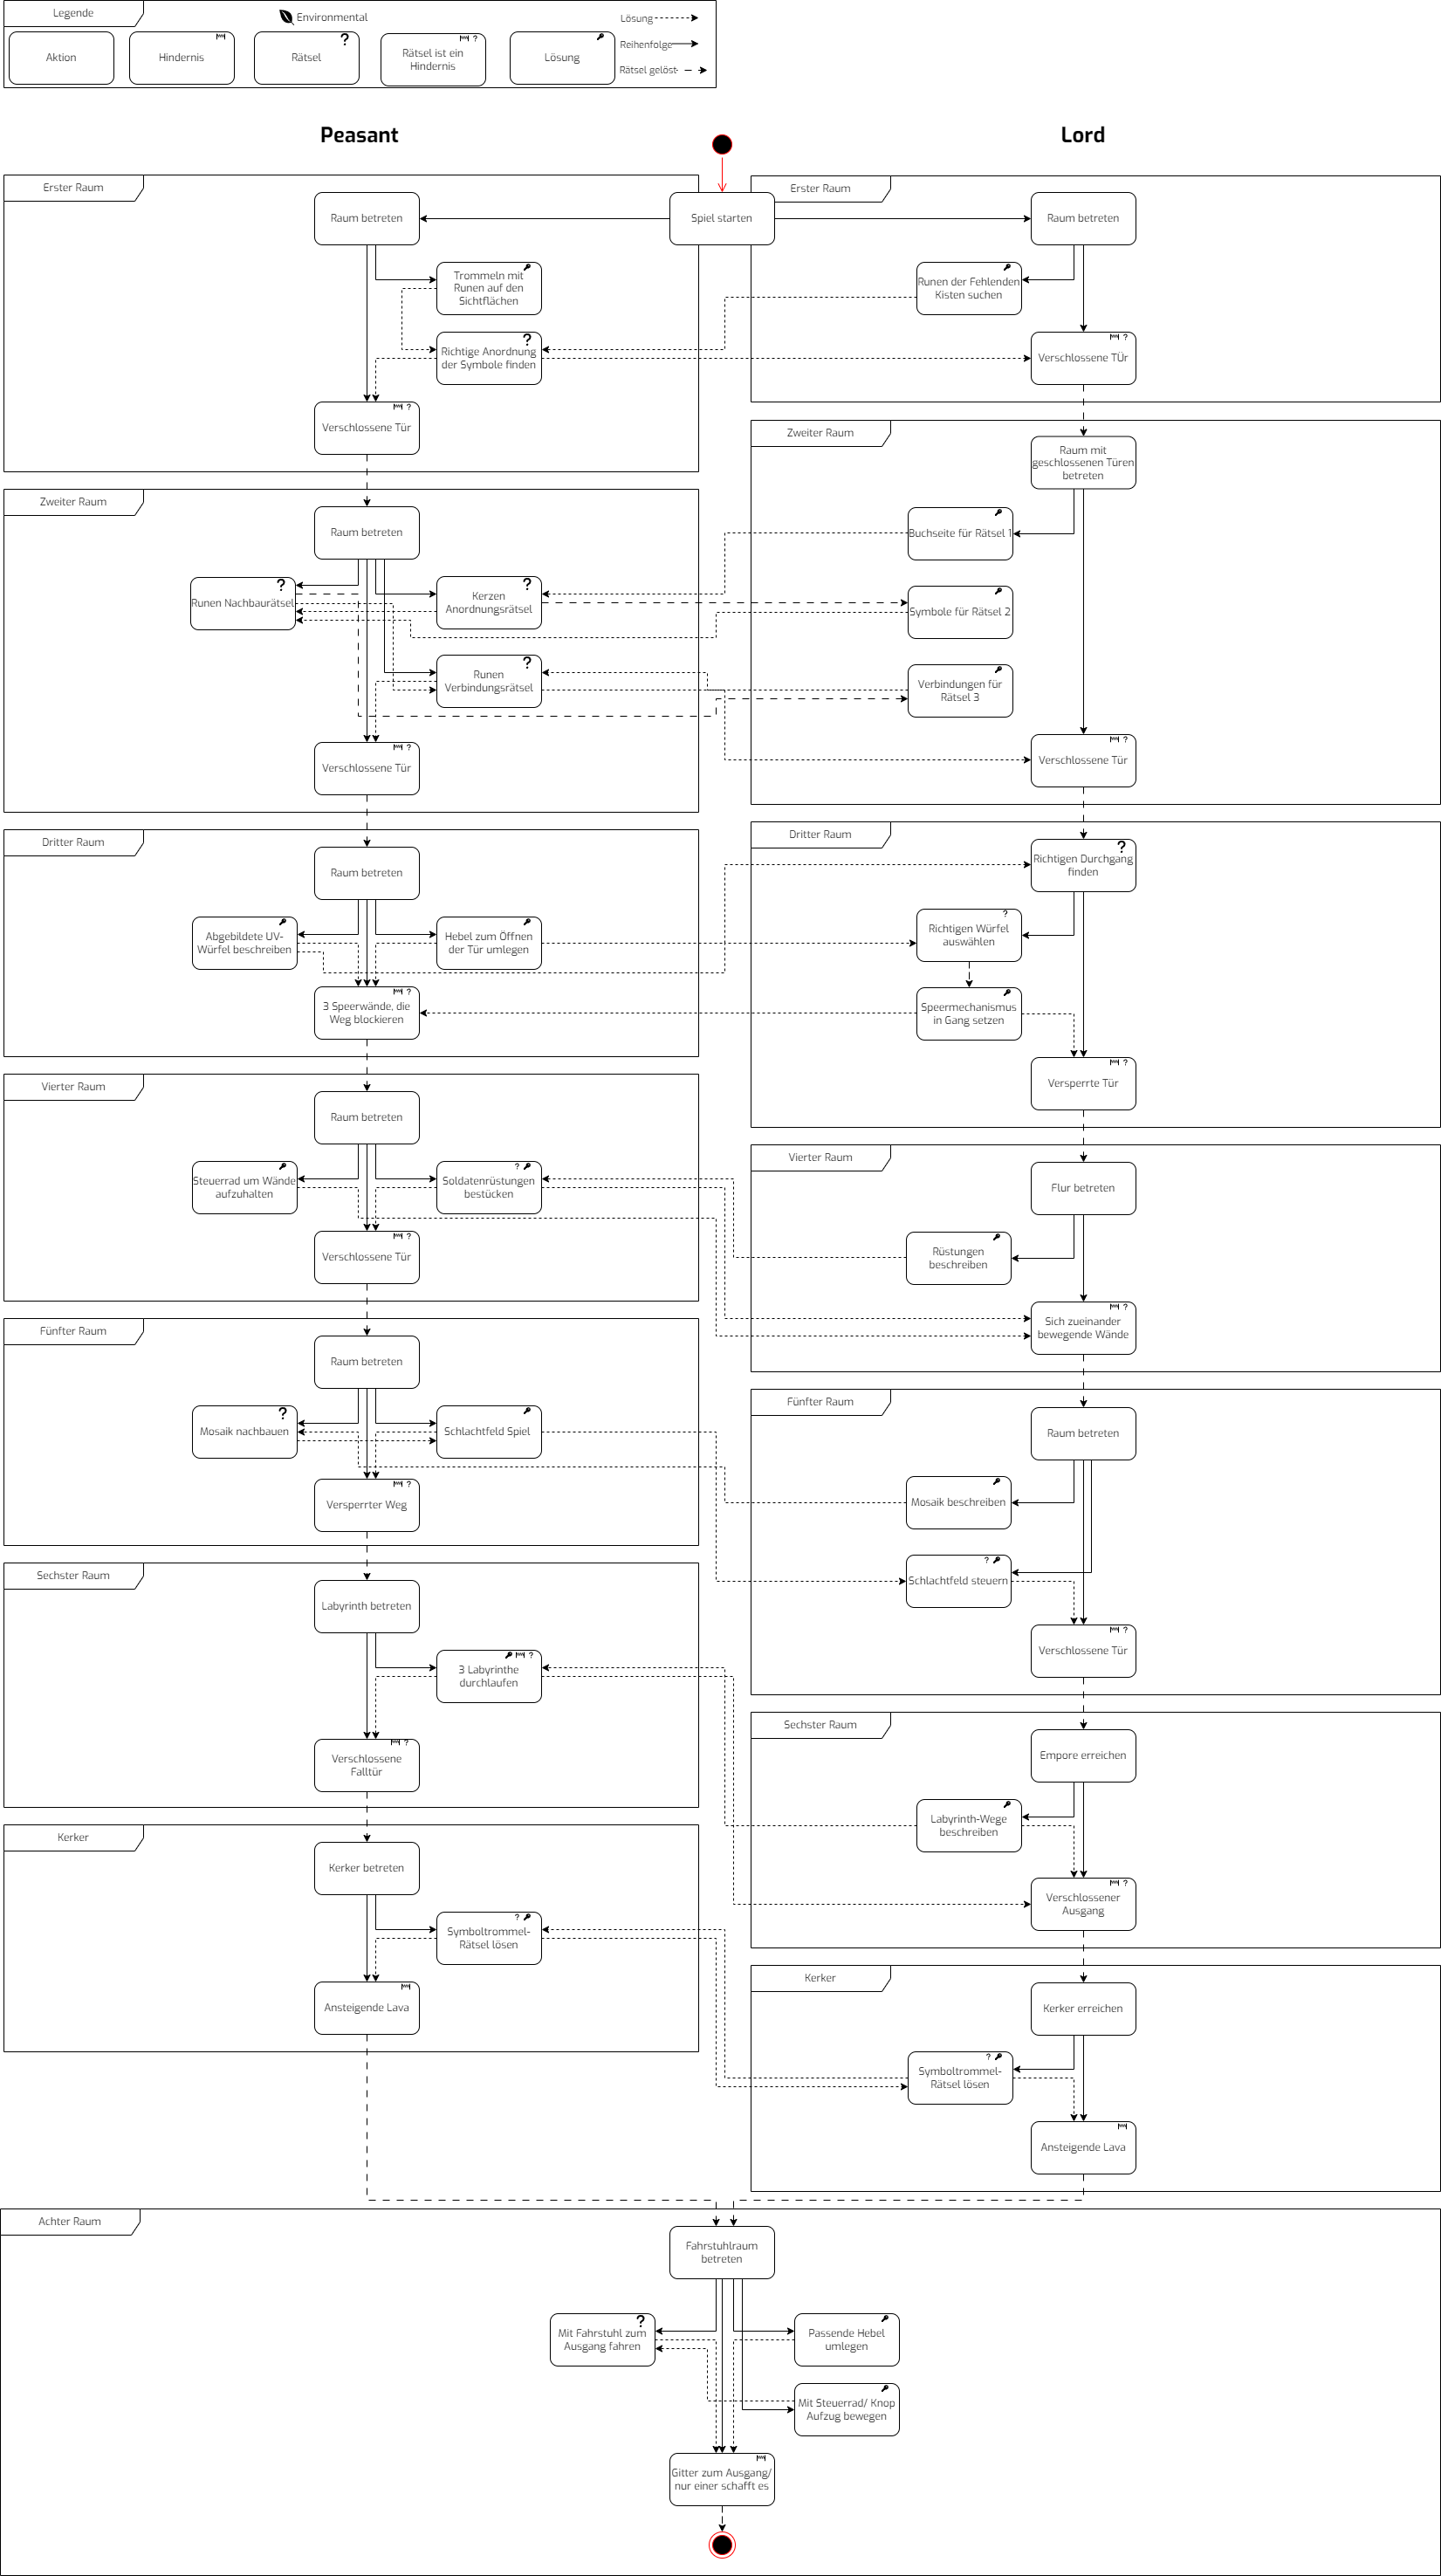
\includegraphics[width=0.8\linewidth]{content/pictures/WeWereHereTooUML.png}
\caption{Rätseldesign von We were here too (Quelle: eigene Darstellung), vollständig in Anhang: }
\label{fig:wwht-uml}
\end{figure}

\paragraph{Schlussfolgerung}
Der zentrale Aspekt der Kommunikationsaufforderung ist in beiden Spielen erkennbar und bildet eine gemeinsame Grundlage. In \say{We were here} fällt jedoch auf, dass das Rätseldesign häufig monoton und eindimensional wirkt - \say{Explorer} stößt auf Rätsel, beschreibt gegebene und/oder gesuchte Gegenstände, \say{Librarian} geht in bestimmten Raum und beschreibt gesuchte Gegenstände, \say{Explorer} löst Rätsel. Es existieren zwar einzelne Ausnahmen, in denen der \say{Librarian} aktiv werden muss um dem \say{Explorer} weiterzuhelfen - \say{Librarian} muss das richtige Ventil vom Rohr öffnen. Doch diese wechselseitige Abhängigkeit bleibt die Ausnahme. Gerade diese Form der Verzweigung ist für \say{Connecting-Minds} essenziell und sollte eine tragende Rolle Spielen. Auf dieser Grundidee lässt sich aufbauen, auch wenn nicht jedes Rätsel in seiner konkreten Ausgestaltung überzeugt, bieten bestimmte Ansätze dennoch wertvolle Anregungen - insbesondere im Hinblick auf die Möglichkeit, abwechslungsreiche, variantenreichere und stärker auf Kooperation ausgelegte Rätsel für \say{Connecting-Minds} zu entwickeln.

Deutlich weiter geht das zweite Spiel, \say{We were here too}, in dem die gegenseitige Verflechtung zwischen den beiden Rollen wesentlich häufiger zum Tragen kommt. In vielen Fällen ist es der \say{Peasant}, der nicht nur seinen eigenen Weg zum nächsten Raum freischaltet, sondern zugleich auch den vom \say{Lord}. In zwei Fällen ist das Prinzip sogar umgekehrt gestaltet: Der \say{Lord} ermöglicht dem \say{Peasant} den Zugang zu neuen Bereichen. In einem der beiden Fällen muss der \say{Peasant} eine Wendeltreppe hinaufrennen, unter der sich der Boden langsam einzieht. Er kommt jedoch nur bis zu einer Schwerwand, die über einen Würfel geöffnet werden kann. Er muss dem \say{Lord} den Aufschnitt des Würfels beschreiben, welcher den richtigen Würfel auswählen muss und in die Zielablage ablegen muss. Durch die Verschachtlung wird der Grundgedanke der Kommunikation und Zusammenarbeit deutlich verstärkt hervorgehoben und erzeugt ausgeglichenen Spaß in den Anwendungen. Ein weiterer Zusatz des Rätseldesigns ist das aufeinander Aufbauen von Rätseln. Dieses Element wird im Rahmen dieser Schlussfolgerung als \say{Mehrstufigkeit} bezeichnet und ist zum Beispiel in Raum 2 zu finden, bei dem aneinander gekettet, verschiedene Rätsel gelöst werden müssen.

Diese strukturelle Ausrichtung eignet sich grundsätzlich gut als gestalterische Vorlage, sofern sie sich sinnvoll in \say{Connecting-Minds} übertragen lässt. Gleichzeitig zielt \say{Connecting-Minds} auf eine noch tiefere und kontinuierliche Abhängigkeit zwischen den beiden Spielerrollen. Beide Rollen sollen nicht nur gelegentlich, sondern regelmäßig und systematisch aufeinander angewiesen sein - die Zusammenarbeit wird damit zur unverzichtbaren Grundlage des Spielfortschritts. Aus der engen Verflechtung ergibt sich, dass Kooperation nicht nur hilfreich, sondern spielentscheidend wird.

Konzepte wie mehrstufige Rätsel oder Einsatz von zeitlichen Begrenzungen (Timer) sind in diesem Zusammenhang ebenfalls interessante Überlegungen. Während Mehrstufigkeit sich als zentrales Element für die Rätselgestaltung anbietet, sollte der Timer gezielt und situationsabhängig eingesetzt werden, da sein Einfluss stark vom jeweiligen Spannungsbogen und dem beabsichtigten Spielerlebnis abhängt.

\subsection{Tiny Room Stories}
Im Vergleich zur \say{We were here}-Reihe ist Tiny Room Stories ein Singleplayer-Spiel bei dem alleine Rätsel gelöst werden müssen, die Abschnitte und Informationen für die Geschichte des Spiels freischalten. Betrachtet wurden in der Analyse der Prolog und Kapitel 1 des Spiels. Der Aufbau der weiteren Kapiteln ist identisch und verändert sich nur im Inhalt des Designs und der Verschachtlung der Rätsel und Hinweise.

\paragraph{Visuelle Analyse}
Die Abbildungen \ref{} und \ref{} in den Anhängen [Anhang verlinken] und [Anhang verlinken] zeigen die Ergebnisse dieser ersten Analyse. Der Fokus liegt zunächst auf den Informationen und Anweisungen die der Spieler vom Spiel erhält. Sie wird fortgesetzt mit der Identifizierung der Rätselarten und wie diese gelöst werden. Außerdem wurde ein Fokus auf die Steuerungshinweise gelegt, um zu bestimmen, welche Steuerungselemente in die Konzeptentwicklung von \say{Connecting-Minds} übernommen werden können. Im allgemeinen besitzt das Spiel \say{Tiny Room Stories} in das Environment eingebettete Rätsel und Hinweise auf die Rätsel. Diese werden ergänzt durch Hinweisnotizen, die das narrative Rätseldesign darstellen. Die zwei Designansätze unterstützen sich gegenseitig und bieten abwechslungsreiche und teilweise herausfordernde Rätsel.

\paragraph{Analyse des Rätseldesigns}
Abbildung \ref{fig:trs-uml} zeigt das Ablaufdiagramm der Rätsel des Spiels. Sowohl in der visuellen Darstellung des Spiels, als auch im Design der Rätsel ist erkennbar, dass Zugänge zu neuen Räumen neue Hinweise oder Rätsel freischalten, welche gelöst werden müssen. Die Rätsel sind dabei gegenseitig verwoben, sodass es oft vorkommt, dass das Lösen von Rätsel A erst Hinweise für Rätsel B zugänglich macht wodurch Rätsel C ebenso gelöst werden kann. Diese Struktur findet sich in Kapitel 1 beim Bücherregal Rätsel wieder, als auch bereits im Prolog beim Öffnen der Schranke.

\paragraph{Schlussfolgerung}
Die Spielsteuerung kann eine gute Vorlage für \say{Connecting-Minds} bietet. Zum einen überzeugt sie durch ihre klare und intuitive Umsetzung, die gut auf diesen Prototyp übertragbar sein kann. Zum anderen passt die Struktur der Rätsel ausgezeichnet zu der Art und Weise, wie die Aufgaben der zwei Spielerrollen gestaltet sein könnten.

Besonders interessant ist dabei, wie sich untergeordnete und übergeordnete Rätsel sinnvoll miteinander verknüpfen lassen: Die Rolle des einen Spielers löst oder entdeckt ein Element, dessen Erkenntnis der andere Spieler anschließend aktiv umsetzen muss, um wiederum des einen Spielers die nächsten Schritte ermöglicht. Dieses Prinzip des wechselseitigen Fortschritt eröffnet spannenden Möglichkeiten für das Rätseldesign von \say{Connecting-Minds}.

\begin{figure}[ht]
\centering
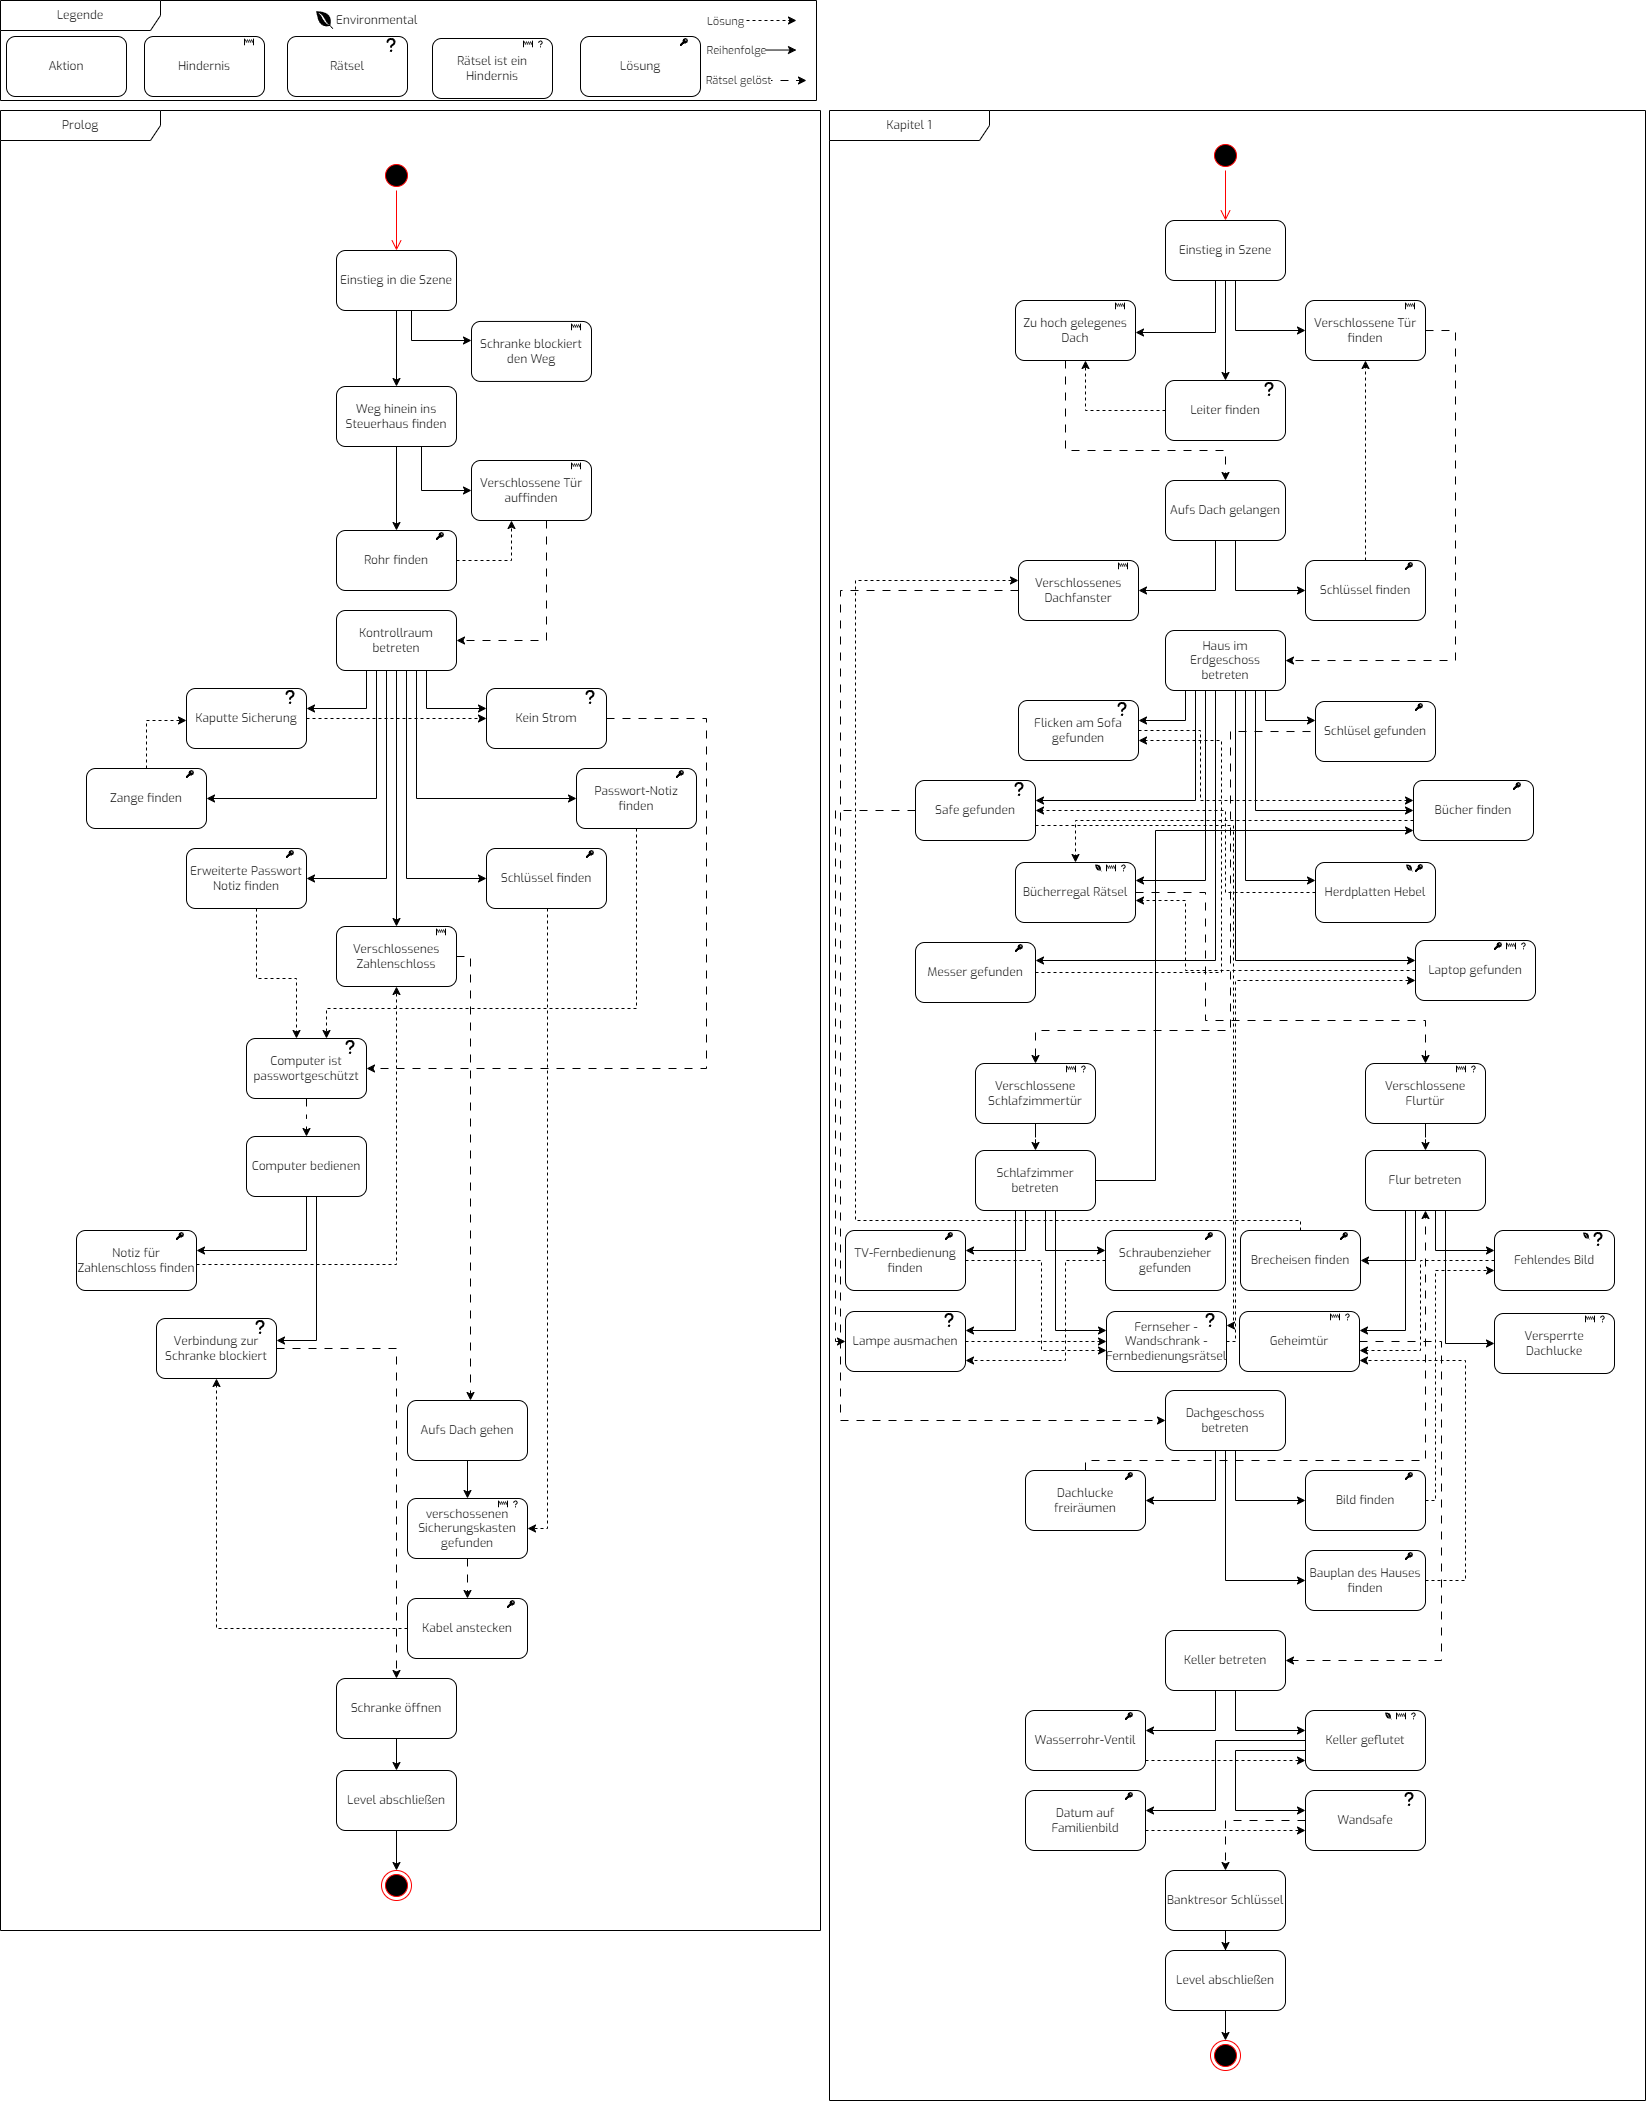
\includegraphics[width=1\linewidth]{content/pictures/TinyRoomStoriesUML.png}
\caption{Rätseldesign von Tiny Room Stories (Quelle: eigene Darstellung), vollständig in Anhang: }
\label{fig:trs-uml}
\end{figure}

\subsection{The past within}

\subsection{Myrmidon}

\subsection{Keep Talking and Nobody Explodes}